\maketitle
\begin{abstract}
A new surface observation can extend an object map while contradicting an earlier object assignment. Treating both updates as a single merge can join unrelated objects; keeping all earlier assignments leaves fragmented objects unresolved. We present a revision module that makes these decisions separately. Historical merges require shared-mask evidence to outweigh separate-object explanations across views, including after removal of any one observation. New measured points are assigned through local competition among object seeds supported by image masks. On two preselected KITTI-360 windows, the method improves mean building/car instance AP50:90 from 17.259 to 18.762. On four further spatial holdouts, AP rises from 20.263 to 23.171, although unconditional revision reaches 23.251. Controlled comparisons attribute the gains to protecting existing identities, consolidating selected fragments, and assigning new points locally. The results also show where conservative merge decisions suppress useful updates. A garage recording demonstrates the same revision module on LiDAR--inertial--visual mapping outputs.
\par\noindent Code: {\urlstyle{same}\url{https://github.com/YanYaoyuan/omni_slam}}.
\end{abstract}

\section{Introduction}
An object mapper may reconstruct the two sides of a building under different identities. A later view can connect their measured surfaces, but geometric connectivity alone cannot determine whether their identities should be merged. The same component may include points from a neighboring structure. A revision rule must distinguish evidence for extending a surface from evidence for changing an established object assignment.

Image-based object mapping systems associate masks across views and accumulate their 3D support~\cite{cg,mc}. Their outputs provide a useful starting map, yet association errors can persist after fusion. Point filtering can remove unsupported geometry; repairing an identity assignment requires deciding which existing object should receive the affected points. This decision becomes particularly important when a broad surface proposal overlaps several persistent objects.

We propose to test historical merges against the observations that support them. For each proposed pair, we compare masks that cover both identities with masks that explain them separately. A merge is permitted only when the shared explanation remains stronger after removing any one jointly observed frame. Pairwise checks within the accepted group prevent a chain of plausible links from joining incompatible objects. A local graph then assigns new measured points and checks whether each proposed historical edit agrees with nearby object evidence. Coordinates remain tied to the original measurements.

We evaluate this revision policy within OmniSLAM, using a fixed object-mapping backbone and pose source. The experiments distinguish the effects of changing old labels, protecting them from an overwrite, and assigning newly added points. We report two prospective KITTI-360 windows separately from four spatial holdouts in previously used sequences. The main gains come from buildings; the ablations and object-level comparisons identify both useful revisions and beneficial merges that the policy rejects.

\begin{figure*}[t]
\centering
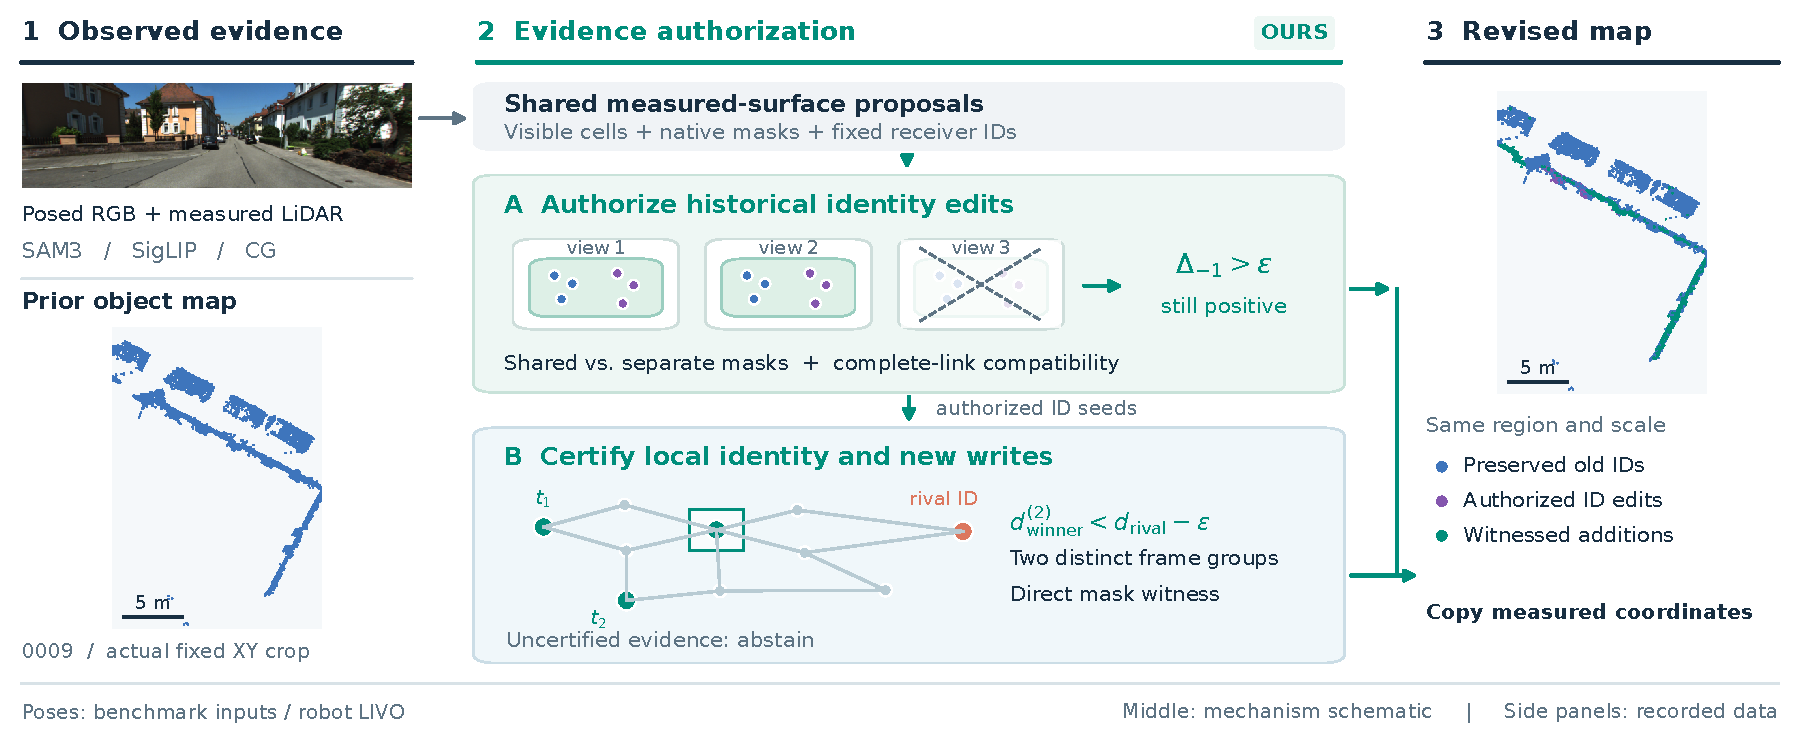
\includegraphics[width=\textwidth]{architecture.pdf}
\caption{Object-map revision. A shared proposal stage selects measured surfaces. Multi-view mask evidence determines which historical identities may merge, and local seed competition determines point assignments. Blue points retain their IDs, purple points change IDs, and teal points are added measurements. The input image and map crops are from KITTI-360 sequence 0009; the middle panels illustrate the decision rules. Map crops share their scale and bounds.}
\label{fig:architecture}
\end{figure*}

\section{Related Work}
\paragraph{Object-centric mapping.}
ConceptGraphs lifts image regions to 3D and associates them into an object graph~\cite{cg}. MaskClustering groups masks using view consensus~\cite{mc}. OVO integrates semantic mapping with SLAM~\cite{ovo}; OVI-MAP separates instance reconstruction from semantic inference~\cite{ovimap}; and VOIM accumulates soft semantic evidence before assigning instances~\cite{voim}. These approaches address how observations form a map. We consider the later revision of point-to-object assignments in a map with persistent identities.

\paragraph{Multi-view refinement.}
Point-Level Refinable Semantic Mapping updates point confidence from temporal mask, depth, and visibility evidence~\cite{refinable}. Our method uses competing mask explanations to test a proposed identity transition, followed by a local check on the affected points. The distinction matters when removing a spurious point and moving a valid point to another object require different actions.

\paragraph{Multimodal fusion.}
FusionMapper combines multimodal and temporal information for vectorized map construction~\cite{jie2025fusionmapper}, while Sparse Deep Interaction Fusion addresses 3D object detection~\cite{yan2025sparse}. We use a fixed perception stack and study the map updates supported by its accumulated observations. SAM3~\cite{sam3}, SigLIP~\cite{siglip}, and SegFormer~\cite{segformer} provide masks, descriptors, and semantic evidence. FAST-LIVO2~\cite{livo} provides poses and measured geometry for the robot experiment.

\section{Object-Map Revision}
\subsection{Map state and surface proposals}
The prior map is $\mathcal M=\{(x_i,o_i)\}$, where $x_i$ is a measured 3D point and $o_i$ is its persistent object ID. The observation archive stores source coordinates, acquisition frames, poses, and image masks. The backbone uses ConceptGraphs-style association with the frozen history2 configuration, SAM3 masks, SigLIP descriptors, and SegFormer semantic evidence. All compared revision variants receive the same prior map and cached observations.

Surface proposals are connected components of a same-class graph on 0.20\,m cells, using 16-neighbor proposals with edge lengths strictly below 0.40\,m. Visible cells contribute equal mass, divided among their projected source pixels. A shared mask-coverage score selects components supported by at least three frames; its full definition is given in Appendix~\ref{app:proposals}. Receivers are fixed by same-class overlap with prior IDs. A component without an old footprint may receive a new ID under the shared source-count and view-support rules. A component that overlaps old objects can only use the proposed existing identities.

\subsection{Historical merge decisions}
A cell represents an old identity only when all its old points have the same nonzero ID. Mixed-ID cells abstain. For identities $a$ and $b$ visible in frame $t$, let $A_{tq},B_{tq}\in[0,1]$ be the fractions of their visible footprint mass covered by same-class query mask $q$, with score $s_{tq}$. We compare a shared-mask explanation with separate explanations:
\begin{align}
S_t(a,b)&=\max_q s_{tq}\min(A_{tq},B_{tq}),\\
E_t(a\mid b)&=\max_q s_{tq}A_{tq}(1-B_{tq}),\\
R_t(a,b)&=\sqrt{E_t(a\mid b)E_t(b\mid a)}.
\end{align}
Let $\delta_t=S_t-R_t$ and $\eps=10^{-10}$. A pair is compatible when
\begin{equation}
\Delta_{-1}(a,b)=\sum_t\delta_t-\max\{0,\max_t\delta_t\}>\eps.
\label{eq:margin}
\end{equation}
This is the minimum margin after removing no frame or any one observed frame. Missing joint views contribute no evidence, and duplicate frame IDs count once.

For each fixed receiver, donor identities are considered in decreasing order of $\Delta_{-1}$, with stable-ID tie breaking. A donor joins the group only if it is compatible with every accepted member. This complete-link rule blocks transitive merging through an incompatible pair. An old point is relabeled only when its donor-to-receiver transition was proposed, the donor was accepted, and the local assignment below agrees with the receiver. Otherwise its old label is retained.

\begin{table*}[t]
\centering
\begin{minipage}[t]{.43\textwidth}\vspace{0pt}\centering\small
\textbf{(a) Prospective windows}\par\smallskip
\begin{tabular}{lrrr}
\toprule
Method & 0009 & 0010 & Mean \\
\midrule
Strong baseline & 23.098 & 11.420 & 17.259 \\
Unconditional & 22.680 & 11.420 & 17.050 \\
History-only & 22.615 & 12.809 & 17.712 \\
\textbf{Ours} & 23.327 & 14.198 & 18.762 \\
\bottomrule
\end{tabular}

\end{minipage}\hfill
\begin{minipage}[t]{.55\textwidth}\vspace{0pt}\centering\small
\textbf{(b) Spatial holdouts in previously used sequences}\par\smallskip
\begin{tabular}{lrrrrr}
\toprule
Method & 0003 & 0004 & 0005 & 0006 & Mean \\
\midrule
Strong baseline & 0.000 & 39.522 & 26.054 & 15.476 & 20.263 \\
Unconditional & 0.000 & 37.309 & 26.778 & 28.917 & 23.251 \\
History-only & 0.000 & 36.200 & 26.778 & 28.917 & 22.974 \\
Witness + history & 0.000 & 38.536 & 26.506 & 26.702 & 22.936 \\
Nearest + history & 0.000 & 38.966 & 26.913 & 26.806 & 23.171 \\
\rowcolor{ourstint}
\textbf{Ours} & 0.000 & 38.966 & 26.913 & 26.806 & 23.171 \\
MaskClustering core & 0.000 & 0.213 & 0.000 & 0.000 & 0.053 \\
\bottomrule
\end{tabular}

\end{minipage}
\caption{Instance AP50:90. The method is fixed across windows. Each mean averages the windows in its own group; missing classes are excluded from a window's class mean. MaskClustering in (b) uses a shared-source core adaptation (Appendix~\ref{app:external}). The nearest-seed control changes only new-point assignment; historical decisions remain those of Ours.}
\label{tab:results}
\end{table*}

\subsection{Local point assignment}
Within an accepted component, pure old-ID cells provide seeds when a selected mask observes them. Approved donors use the receiver's identity; other old identities remain separate. Components with no old footprint use their proposed new identity at witnessed cells. Each seed retains the frame that supports it.

Let $d_o(v)$ be the shortest-path distance from node $v$ to seeds of identity $o$. For the unique nearest identity $o^*$, let $d^{(2)}_{o^*,t}(v)$ denote its second-nearest distance from a distinct seed-frame group. The assignment passes the stability check when two such groups exist and
\begin{equation}
d^{(2)}_{o^*,t}(v)<\min_{o\ne o^*}d_o(v)-\eps.
\label{eq:certificate}
\end{equation}
Deleting any one seed-frame group then leaves a winning seed closer than every competing identity. This property assumes a fixed graph and edge weights; it does not imply that the winning label is semantically correct.

A new point is admitted when its component is accepted, its cell has direct mask support, and Eq.~\ref{eq:certificate} supplies an identity. Support is checked at cell level, so another measurement in the same 0.20\,m cell may be admitted. Coordinates are copied from the measurement archive. The shared proposal stage excludes additions within 0.05\,m of prior geometry. All variants inherit the same class scores and receive no additional variant-specific filtering. The effect of the stability check is separated from nearest-seed assignment in the experiments.

\begin{figure*}[t]
\centering
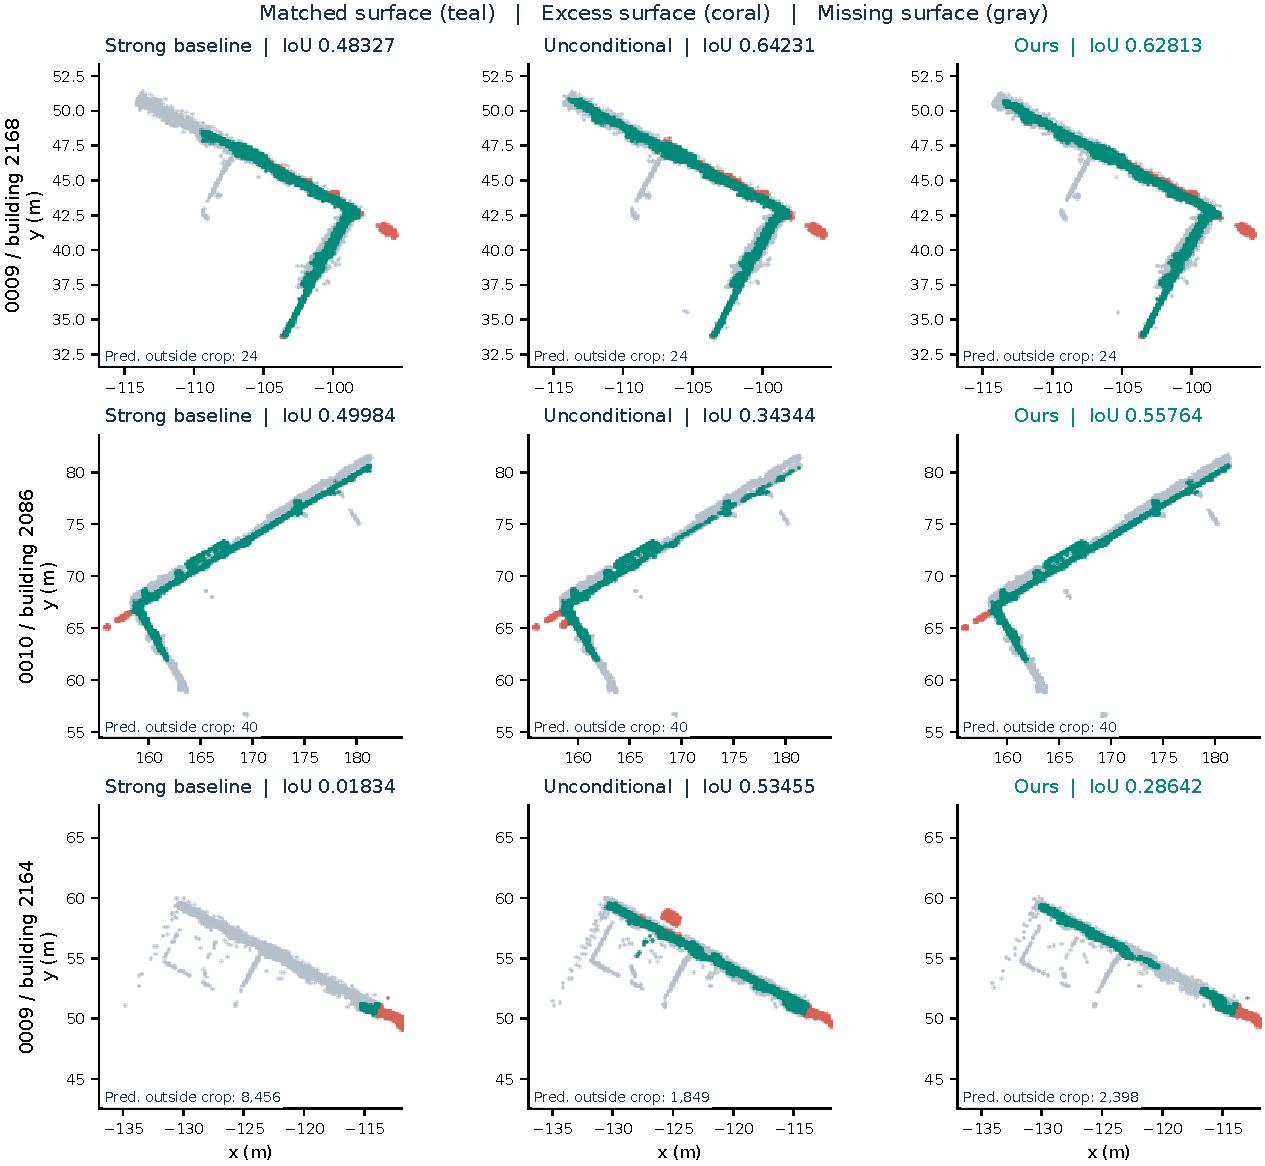
\includegraphics[width=.82\textwidth]{object_cases.pdf}
\caption{Two improved building reconstructions and a rejected useful update. Teal denotes correct target support, coral excess surface, and gray missed surface. Crops share bounds within each row; IoU is computed over the full confidence-weighted reference domain. For building 2164, unconditional revision reaches IoU 0.535 and Ours reaches 0.286. These cases were selected after scoring to examine the revision decisions.}
\label{fig:cases}
\end{figure*}

\section{Experiments}
\subsection{Data and evaluation}
We evaluate building and car instances on KITTI-360~\cite{kitti}. The prospective comparison uses sequence 0009, frames 778--1026 (50 sampled image--LiDAR pairs), and sequence 0010, frames 1872--2033 (34 pairs). Seven development-exposed sequences were excluded in full, and the windows and method were fixed before image processing and semantic-reference decoding. A second comparison uses four spatial holdouts from previously exposed sequences 0003--0006, with 61 pairs each. These two groups are reported separately. Geometry weights were fitted on development data from 0000/0002 and remain fixed throughout.

We transfer predicted IDs to the full static reference domain using the nearest map point within a strict 0.20\,m radius. A local confidence-weighted adapter calls the public AP kernel with the upstream train-ID reference encoding. AP is averaged over IoU thresholds 0.50, 0.55, $\ldots$, 0.90, with a minimum reference confidence mass of 100. The two prospective windows contain 83 eligible instances, including uncovered objects. All AP values are percentages. This protocol evaluates local maps and is not an official test-server submission. Appendix~\ref{app:protocol} gives the selection and scoring details.

\paragraph{Controls.}
The strong baseline is the frozen object map. Unconditional revision applies all shared component assignments. History-only applies the authorized old-label changes while keeping every parent-added point, label, and score. \ours{} also applies the local admission and assignment policy. These controls share perception outputs and surface proposals. A MaskClustering core adaptation is reported separately because its mask inputs and semantic readout differ from the native method.



\subsection{Map accuracy}
On the prospective windows, \ours{} reaches 18.762 mean AP, compared with 17.259 for the strong baseline and 17.712 for history-only (Table~\ref{tab:results}a). AP50 rises from 33.453 to 34.319 in 0009 and from 18.056 to 30.556 in 0010. The canonical-class and uniform-score checks also improve, indicating that the gain is not solely a change in ranking scores (Appendix~\ref{app:protocol}).

Two additional buildings, 2168 and 2086, cross the AP50 threshold without losing an existing match. Both were partially covered by the baseline. For 2086, IoU moves from 0.49984 to 0.55764, so one added match starts immediately below the threshold. Figure~\ref{fig:cases} shows these gains alongside building 2164, for which unconditional revision produces a better completion.

On the four spatial holdouts, mean AP increases from 20.263 to 23.171. Four canonical AP50 matches are gained and none are lost. However, unconditional revision reaches 23.251, and \ours{} falls by 0.557 AP points relative to the baseline in 0004. The gains over the backbone therefore extend to another set of locations, while the relative benefit of conservative revision varies across windows.



\subsection{Effects of revision decisions}
We use five post-hoc output interventions per prospective window to separate historical relabeling from new-point assignment. Each copies fixed predictions and changes only the designated labels or admitted sources. Table~\ref{tab:causal} compares paired interventions; the complete definitions and scores are in Appendix~\ref{app:causal}.

\begin{table}[t]
\centering\footnotesize
\begin{tabular}{@{}lrrr@{}}
\toprule
AP difference (pp) & 0009 & 0010 & Mean \\
\midrule
Apply authorized old edits & +0.161 & +0.000 & +0.081 \\
Protect vs. unconditional & +0.073 & +2.778 & +1.426 \\
Local policy vs. witness & +0.097 & +1.389 & +0.743 \\
New certificate vs. nearest & +0.000 & +0.000 & +0.000 \\
\bottomrule
\end{tabular}

\caption{AP differences between paired output interventions. Historical-label contrasts hold new coordinates, labels, and scores fixed; new-point contrasts hold historical decisions fixed. Rows are conditional effects and are not additive.}
\label{tab:causal}
\end{table}

\paragraph{Historical edits and preservation.}
In 0009, applying the authorized old-label changes adds 0.161 AP points relative to preserving the old labels at the same new geometry. A fixed baseline-to-reference correspondence identifies the changes as consolidation of fragments belonging to the same building. In 0010, \ours{} changes no historical labels, yet preserving them instead of applying unconditional edits adds 2.778 points. Protecting an existing assignment can thus account for a gain even when no historical edit is executed.

\paragraph{New-point assignment.}
Local assignment improves mean AP by 0.743 points over direct mask-supported admission with parent labels. Removing the extra seed-frame stability requirement gives exactly the same AP as \ours{} in all six evaluation windows. In 0009, the check excludes 35 additional sources and changes five reference labels; in 0010, it changes neither. The observed benefit comes from local identity assignment, with no measured AP increment from the additional check.

\subsection{Failure cases and scope}
Conservative merging leaves some correct completions unfinished, as building 2164 illustrates. On 0009, best same-class object IoU improves for 15 canonical objects, declines for 26, and is unchanged for 21; the corresponding counts in 0010 are 2, 0, and 10. Unchanged AP50 match counts therefore conceal some geometric regressions. Car AP in 0010 remains 6.173 for all four primary methods, and car AP in 0009 falls from 45.411 to 45.355. Building improvements dominate the aggregate gain.

Development results are also reported in Appendix~\ref{app:development}: mean AP is 28.012 for the strong baseline, 28.048 for \ours{}, and 28.217 for history-only. That comparison did not meet the original development criterion. The prospective evaluation and spatial extension retain their separate selection rules and outcomes.

\subsection{Garage integration}
We applied the same revision code to 330 frames of \texttt{rosbag2245}, using the existing LIVO poses and point archive. \ours{} produces 717,816 points and 68 nonempty IDs while retaining all old labels. Appendix~\ref{app:robot} shows the four-method comparison with recorded images. This offline run uses the complete measurement archive; the public-data adapter respects source acquisition time. Without independent garage annotations, the comparison demonstrates integration but does not measure semantic accuracy.

\section{Conclusion}
Historical relabeling and surface expansion have different failure modes. Testing them separately improves the evaluated object maps through selective fragment consolidation, identity preservation, and local assignment of new measurements. The policy can also reject useful merges, and its additional seed-frame check provides no AP gain over nearest-seed assignment. Evaluation remains limited to local KITTI-360 windows and an unannotated robot recording. Native full-system comparisons, longer sequences, and pose/depth perturbations are needed to assess broader applicability. The current proposal representation also limits recovery: an incorrect old footprint can prevent creation of a new identity inside that component.

\balance
\begingroup
\small
\setlength{\bibsep}{1pt}
\bibliographystyle{unsrtnat}
\bibliography{references_current}
\endgroup
